\section{Arduino}
Den indledende løsning blev først implementeret på en Arduino Uno mikrocontroller hvorefter konceptet blev testet og verificeret. Koden er derfor i sin indledende fase også skrevet i Arduino.

\begin{figure}[h!]
  \centering
  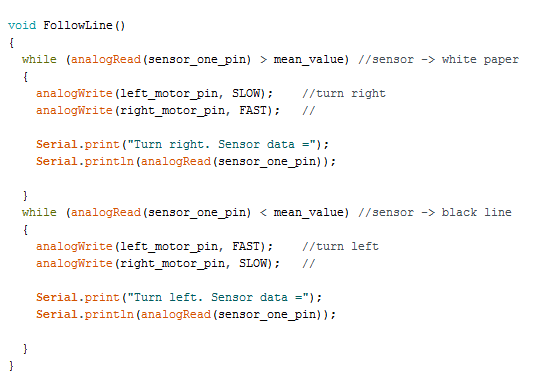
\includegraphics[width=0.6\textwidth]{figures/followLine2.png}
  \caption{FollowLine() funktion.}
  \label{follow_line_kode}
\end{figure}

På overstående figur ses funktionen follow\_Line(). Koden fungerer sålades at når sensoren registrerer den hvide omkringliggende farve drejes der til højre og når den sorte linje registreres drejes der til venstre. Robotten kører derved kun på kanten af linjen. 

\subsection{Test og delkonklussion}
Ud fra det introducerde linetrack system blev konceptet testet ved brug af én sensor på den opstillede bane. 
\newline
Ud fra denne test kan det konkluderes at softwaren virker i henhold til den indledende problemløsning. Robotten er i stand til at følge kanten af linjen ved hjælp af de forskellige overfladefarveværdier som sensoren registrerede gennem testen. 
\newline

\begin{figure}[h!]
  \centering
  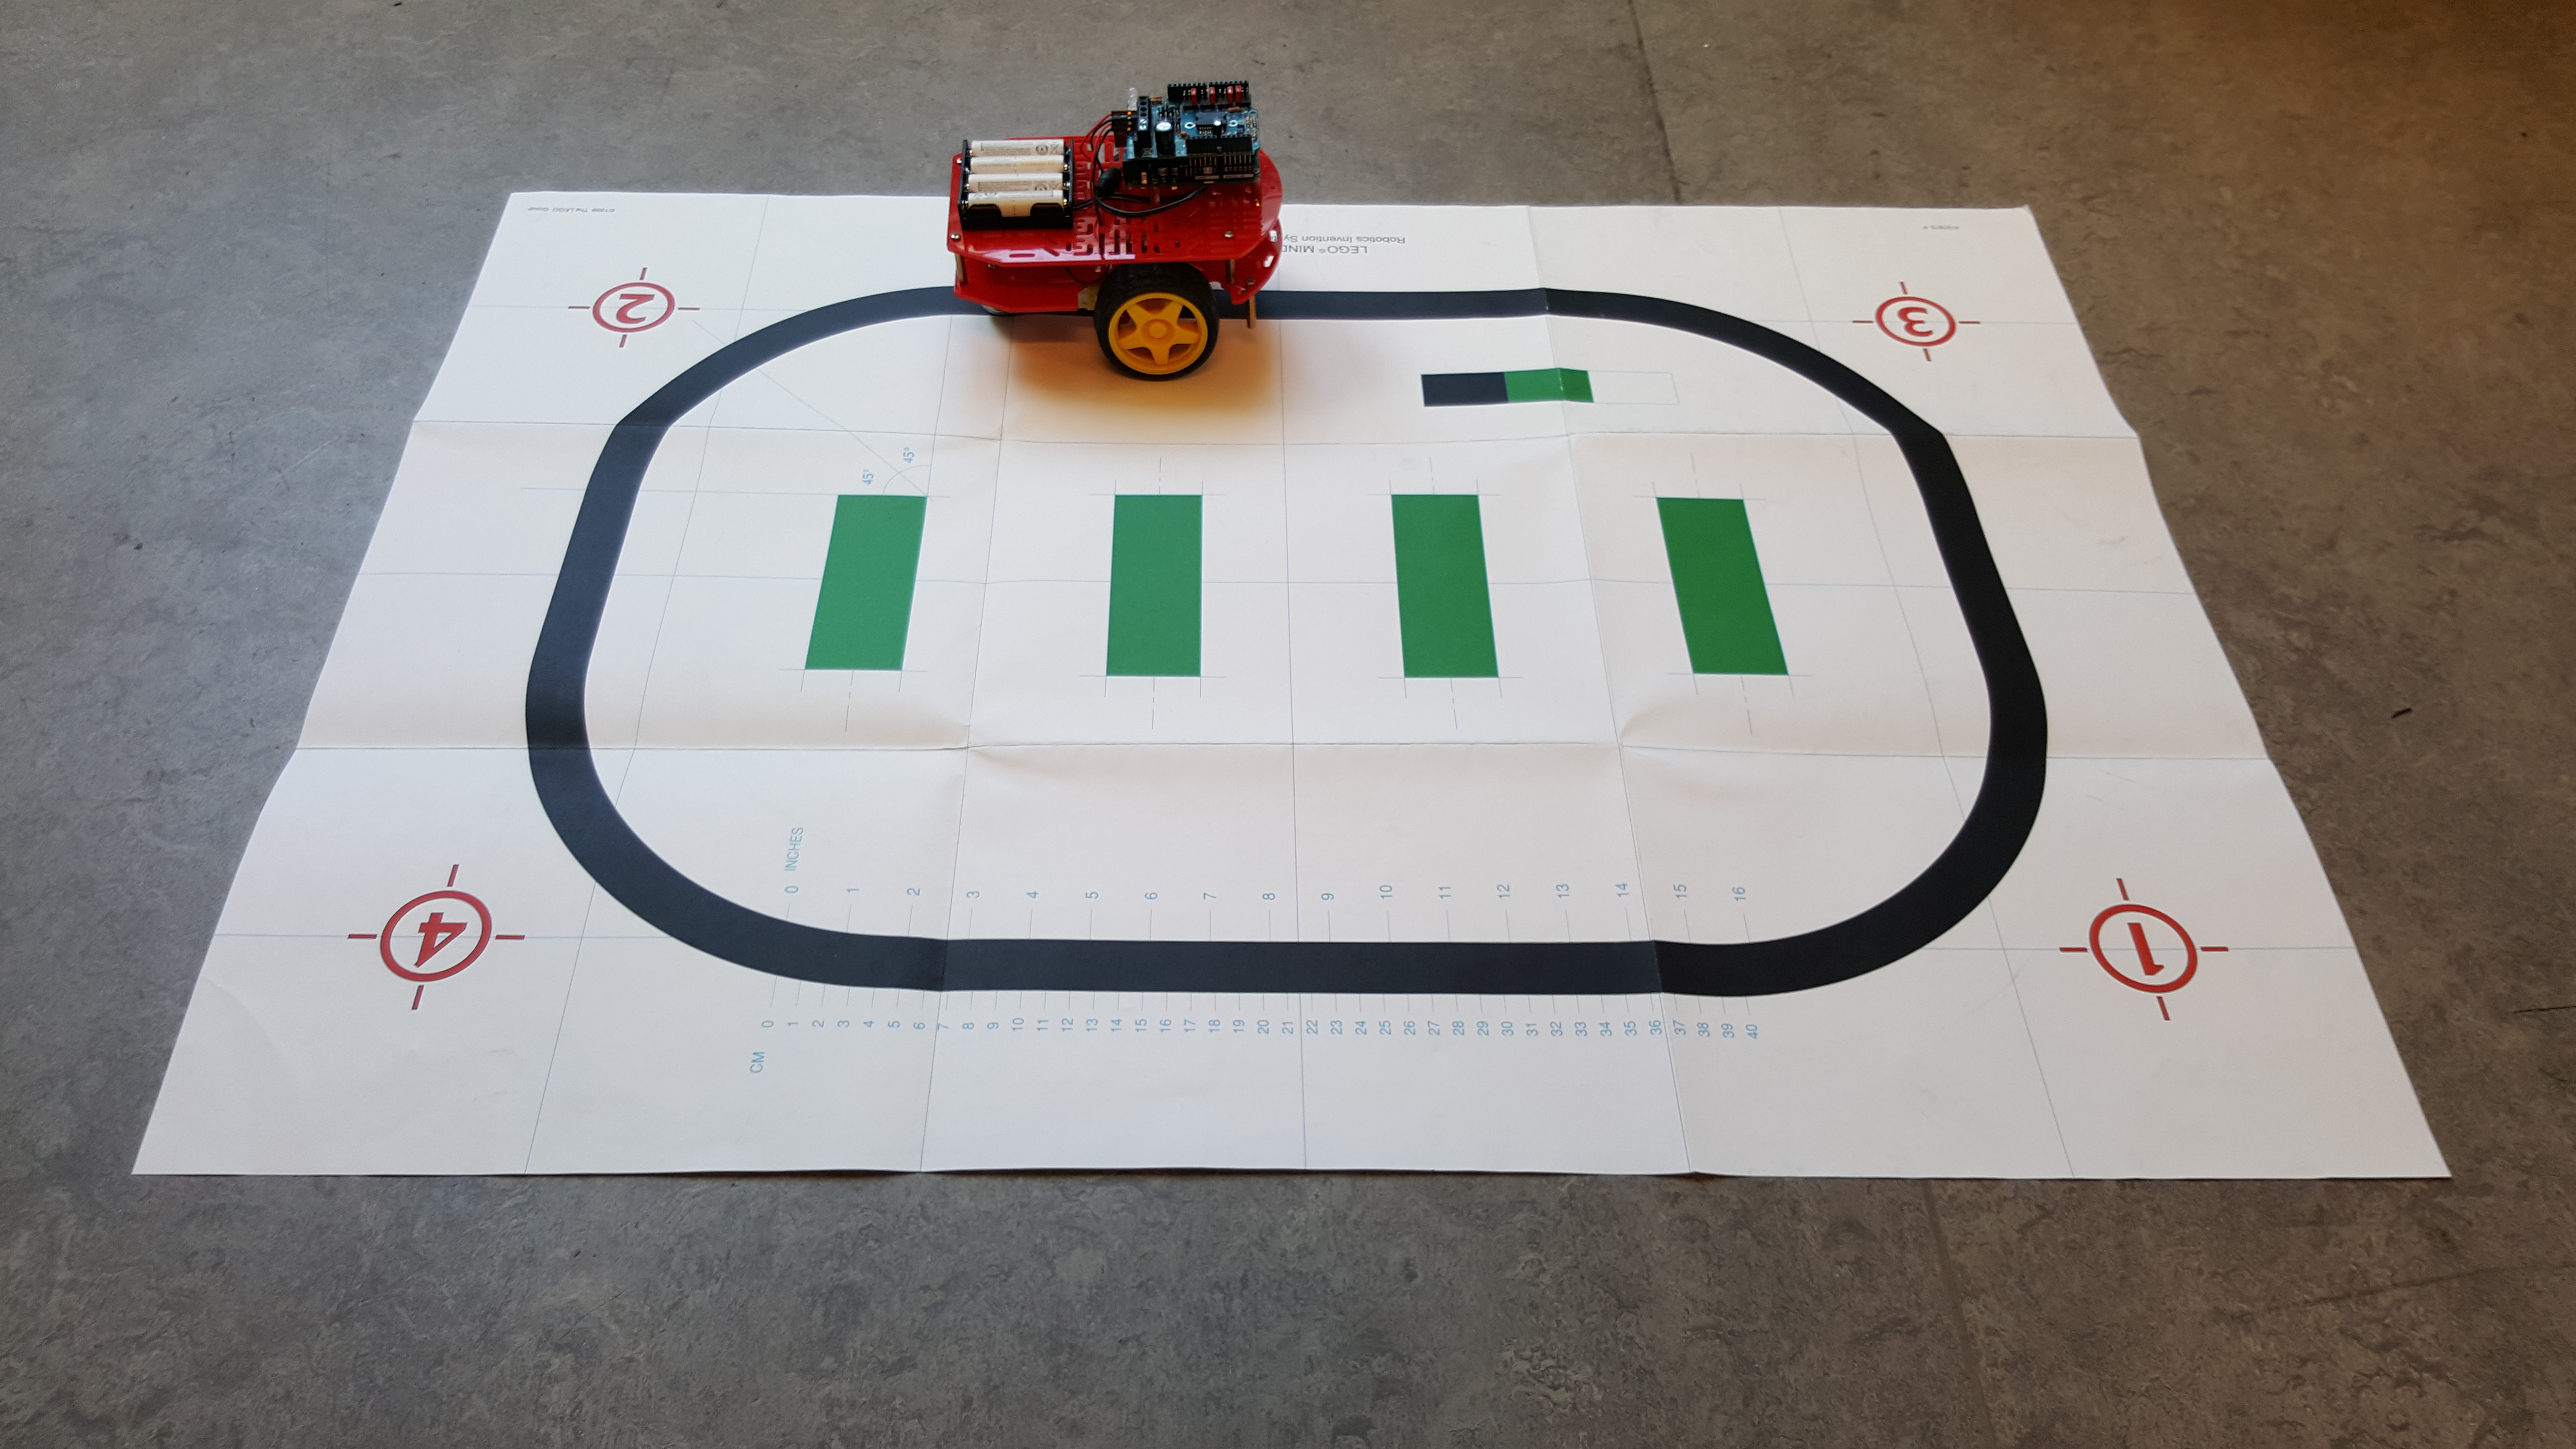
\includegraphics[width=0.6\textwidth]{figures/testMedEnSensor.png}
  \caption{Den inledende software løsning til linetrackinging med 1 sensor.}
  \label{init_software}
\end{figure}


